\beginsong{Burschen, Burschen}[
    wuw={bündische Jugend}, 
    bo={46}, 
    pfii={20}, 
    pfiii={12}, 
    gruen={158}, 
    siru={36},
    tonspur={176}, 
]

\beginverse
\endverse
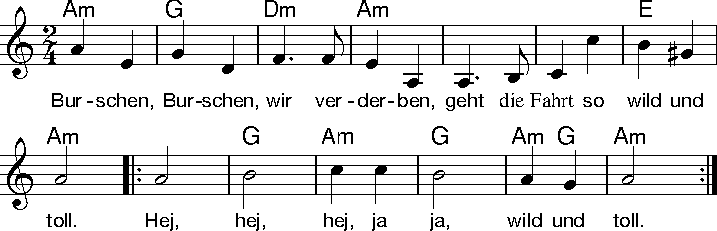
\includegraphics[draft=false, width=1\textwidth]{Noten/Lied012.pdf}

\beginverse
\[Am]Von den \[G]Füßen \[Dm]weg\[Am]gesoffen 
werden bald die \[E]Stiefel \[Am]sein,
\lrep \[Am]hej, \[G]hej, \[Am]hej, ja\[G]ja, \[Am]Stie\[G]fel \[Am]sein.\rrep
\endverse
 
\beginverse
^Eine ^Nacht, ^zwei tol^le Tage 
zechten wir an ^diesem ^Ort,
\lrep ^hej, ^hej, ^hej, ja^ja, ^die^sem ^Ort. \rrep
\endverse

\beginverse
^Zechen ^wir an ^diesem ^Orte, 
hier in diesem ^blauen ^Krug,
\lrep ^hej, ^hej, ^hej, ja^ja, ^blau^en ^Krug.\rrep
\endverse

\beginverse
^Süß das ^Bier und ^weiß ^die Kannen, 
schön die flinke ^Krüger^in.
\lrep ^hej, ^hej, ^hej, ja^ja, ^Krü^ger^in. \rrep
\endverse

\beginverse
^Sauft das ^Bier, zer^schlagt die ^Kannen, 
küsst die schöne ^Krüger^in,
\lrep ^hej, ^hej, ^hej, ja^ja, ^Krü^ger^in.\rrep
\endverse

\endsong
